\documentclass[11pt]{article}

\usepackage{pablo}
\usepackage{multicol}
\usepackage[a5paper,margin=1.5cm]{geometry}
\usetikzlibrary{calc}
%\tikzset{math3d/.style= {y= {(1,0)}, z={(0,1)},x={({-cos(30)},{-sin(30)})}}}
\tikzset{math3d/.style= {x= {(-0.866cm,-0.5cm)}, z={(0cm,1cm)},y={(1cm,0cm)}}}
\pagestyle{empty}

\begin{document}

\begin{center}
  \textsc{Devoir} --- Espace \& Probabilités
\end{center}
\hrule

\begin{exercice}[Définitions --- 4 points]\emph{Sauf mention contraire, on ne demande pas de justifier.}

  On lance un dé à 10 faces (numérotées de 1 à 10) équilibré, et on s'intéresse au nombre obtenu.
  \begin{enumerate}
    \item L'évènement «~Obtenir un nombre pair~» est-il un évènement élémentaire ?
    \item Quelle est la probabilité de l'évènement «~Obtenir 9 ou 10~» ? Justifier.
    \item
      \begin{enumerate}
      \item Si cela est possible, proposer un évènement qui a une probabilité de 0,4 ; si c'est impossible, expliquer pourquoi.
      \item Même question avec une probabilité de 1,1.
    \end{enumerate}
    \item Soit l'évènement $A$ : «~Obtenir un nombre impair~».
        Proposer un évènement incompatible avec $A$.
    \item Donner les issues correspondant à l'union des évènements «~Obtenir un multiple de 3~» et «~Obtenir un nombre supérieur à 7~».
  \end{enumerate}
\end{exercice}

\begin{exercice}[3 points]
  Soient $A$ et $B$ deux évènements tels que $P(A)=0,4$, $P(B)=0,2$, et $P(A\cap B)=0,1$.
  \begin{enumerate}
    \item Calculer $P(\bar A)$.
    \item Calculer $P(A\cup B)$.
  \end{enumerate}
\end{exercice}

\begin{exercice}[Tableau --- 5 points]
  Une urne contient des boules blanches ou noires, et chacune porte un des deux numéros 1 ou 2. On sait qu'en prenant une boule au hasard, il y a une probabilité de :
  \begin{itemize}[$\bullet$]
    \item 55\% d'avoir une boule noire (indépendamment du numéro) ;
    \item 15\% d'avoir une boule blanche portant le numéro 1 ;
    \item 10\% d'avoir une boule noire numérotée 1.
  \end{itemize}

  \begin{multicols}{2}
  \begin{enumerate}
    \item Reproduire sur votre copie le tableau ci-contre, et complétez le avec les probabilités des différents évènements.
  \end{enumerate}

  \columnbreak

  \begin{center}
  \begin{tabular}{p{1.2cm}|p{0.8cm}|p{0.8cm}|p{0.9cm}}
  & N\up{o} 1 & N\up{o} 2 & Total \\
  \hline
  Blanche & & & \\
  \hline
  Noire   & & & \\
  \hline
  Total   & & & \\
\end{tabular}
\end{center}
\end{multicols}
\begin{enumerate}
    \setcounter{enumi}{1}
    \item Quelle est la probabilité d'avoir une boule noire portant le numéro 2 ?
    \item Quelle est la probabilité de l'évènement «~Tirer une boule noire ou numérotée 2~» ?
    \item Quel évènement a une probabilité de 30\% ?
  \end{enumerate}
\end{exercice}

\begin{exercice}[Boule --- 6 points]\emph{Toutes les longueurs sont données en centimètres.}

  \begin{multicols}{2}
    \noindent On considère le parallélépipède rectangle $ABCDEFGH$ représenté ci-contre (la figure n'est pas à l'échelle), avec les longueurs $AB=6$, $BC=6$, $BF=3$.

  \begin{center}
  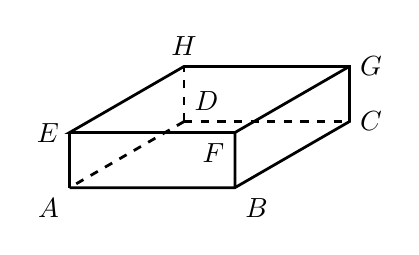
\begin{tikzpicture}[scale=0.7,line width=1pt]
    \coordinate (O) at (0,0);
    \coordinate (x) at (3,0);
    \coordinate (y) at ({3*0.8*cos(30)},{3*0.8*sin(30)});
    \coordinate (z) at (0,1);

    \coordinate (A) at (O);
    \coordinate (B) at ($(O) + (x)$);
    \coordinate (C) at ($(O) + (x) + (y)$);
    \coordinate (D) at ($(O) + (y)$);
    \coordinate (E) at ($(O) + (z)$);
    \coordinate (F) at ($(O) + (z) + (x)$);
    \coordinate (G) at ($(O) + (z) + (x) + (y)$);
    \coordinate (H) at ($(O) + (z) + (y)$);

    \draw (A) node[below left]{$A$};
    \draw (B) node[below right]{$B$};
    \draw (C) node[right]{$C$};
    \draw (D) node[above right]{$D$};
    \draw (E) node[left]{$E$};
    \draw (F) node[below left]{$F$};
    \draw (G) node[right]{$G$};
    \draw (H) node[above]{$H$};
    \draw (A) -- (B) -- (C) -- (G) -- (H) -- (E) -- (F) -- (B);
    \draw (A) -- (E);
    \draw (F) -- (G);
    \draw[dashed] (D) -- (H);
    \draw[dashed] (D) -- (A);
    \draw[dashed] (D) -- (C);
  \end{tikzpicture}

\end{center}
\end{multicols}

Le but de l'exercice est de déterminer le volume de la boule circonscrite à ce solide (c'est-à-dire la plus petite boule pouvant contenir ce solide). On admet que le segment $[AG]$ est le diamètre de cette boule.

\begin{enumerate}
  \item Calculer la longueur du segment $[AC]$.
  \item En admettant que $ACG$ est rectangle en $C$, montrer que $AG=9$.
  \item En déduire le volume de la boule circonscrite à $ABCDEFGH$.
\end{enumerate}
\end{exercice}

\begin{exercice}[Exercice ouvert --- 2 points]\emph{Toute trace de recherche, même incomplète, sera prise en compte dans la notation.}
  \begin{multicols}{2}
  \noindent On considère le cube $ABCDEFGH$, de côté 2~cm. Le point $I$ est le centre de la face $AEFB$ ; $J$ est le centre de la face $CGFB$. Quelle est la longueur du segment $[IJ]$ ?

  \begin{center}
  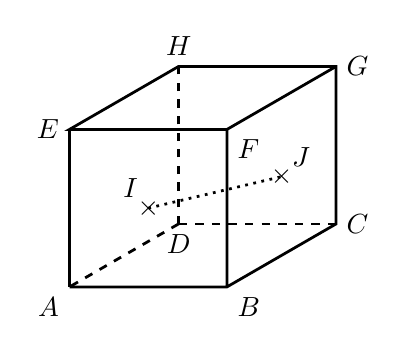
\begin{tikzpicture}[scale=2,line width=1pt]
    \coordinate (O) at (0,0);
    \coordinate (x) at (1,0);
    \coordinate (y) at ({0.8*cos(30)},{0.8*sin(30)});
    \coordinate (z) at (0,1);

    \coordinate (A) at (O);
    \coordinate (B) at ($(O) + (x)$);
    \coordinate (C) at ($(O) + (x) + (y)$);
    \coordinate (D) at ($(O) + (y)$);
    \coordinate (E) at ($(O) + (z)$);
    \coordinate (F) at ($(O) + (z) + (x)$);
    \coordinate (G) at ($(O) + (z) + (x) + (y)$);
    \coordinate (H) at ($(O) + (z) + (y)$);
    \coordinate (I) at ($(O) + 0.5*(x) + 0.5*(z)$);
    \coordinate (J) at ($(O) + (x) + 0.5*(y) + 0.5*(z)$);

    \draw (A) node[below left]{$A$};
    \draw (B) node[below right]{$B$};
    \draw (C) node[right]{$C$};
    \draw (D) node[below]{$D$};
    \draw (E) node[left]{$E$};
    \draw (F) node[below right]{$F$};
    \draw (G) node[right]{$G$};
    \draw (H) node[above]{$H$};
    \draw (A) -- (B) -- (C) -- (G) -- (H) -- (E) -- (F) -- (B);
    \draw (A) -- (E);
    \draw (F) -- (G);
    \draw[dashed] (D) -- (H);
    \draw[dashed] (D) -- (A);
    \draw[dashed] (D) -- (C);

    %\draw[dotted] (A) -- (F) -- (C);
    \draw (I) node{$\times$} node[above left]{$I$};
    \draw (J) node{$\times$} node[above right]{$J$};
    \draw[dotted] (I) -- (J);
  \end{tikzpicture}
\end{center}
\end{multicols}
\end{exercice}


\end{document}

